\section{Process development and flowsheeting}

\subsection{Process overview}

Nitroma's process for the production of substituted aromatic amines via nitration is composed of four section, as shown in \Cref{fig:BFD}: toluene nitration (red); o-nitrotoluene reduction (green); p-nitrotoluene partial oxidation and nitrobenzaldehyde reduction (purple); p-nitrotoluene complete oxidation and nitrobenzoic acid reduction (blue). 


\begin{figure}[H]
    \centering
    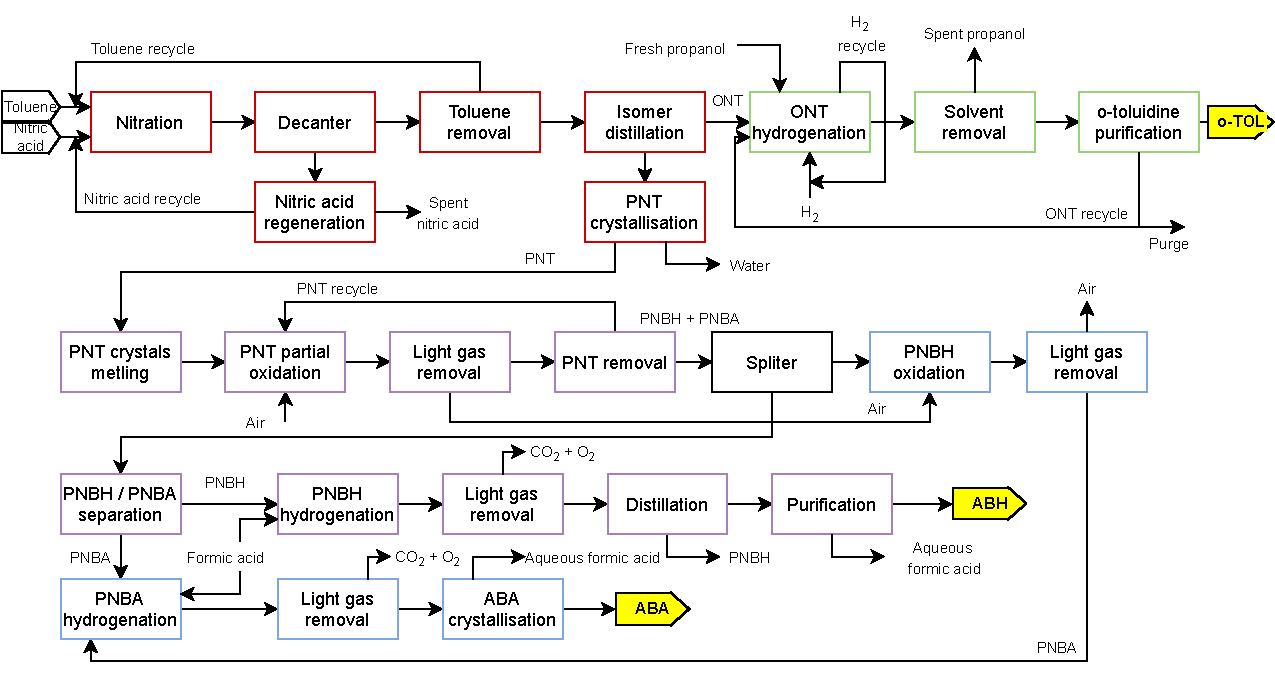
\includegraphics[width=\linewidth]{1-Figures/BFD_nitroma.pdf}
    \caption{Block Flow Diagram of Nitroma's process}
    \label{fig:BFD}
\end{figure}

Following the selection of separation techniques and reactor types for each step shown in \Cref{fig:BFD}, the process was simulated with ASPEN Plus to obtain approximates for sizing, heat duties and residence times required to meet the production targets. Reaction kinetics were modelled as Arrhenius rate laws with constants and activation energies derived from published work. The thermodynamic property method xx was selected because xx
For a plant operating at steady-state 310 days per year, ASPEN simulations found that 626 tonnes/year of 99\% pure o-Toluidine, 500 tonnes/year of 99.3\% pure Aminobenzaldehyde and 107 tonnes/year of pure Aminobenzoic acid could theoretically be produced by Nitroma's process.

This section will detail the decision making steps taken to determine the optimum reactor types and separation strategies for the development of an inherently safe and continuous process. Particular importance was given to process intensification principles during technology selection, which gave rise to process innovations.


\subsubsection{Operating mode} % batch vs continuous
The first level of decision according to \textcite{douglas_conceptual_1988} is whether to operate a batch or continuous process. On the one hand, a continuous process is designed to operate at almost constant conditions 24 hr/day for 7 days/week until the plant is shut down for planed maintenance. On the other hand, batch processes are made of several units designed to be started and stopped frequently. Most processes contain a mix of batch and continuous units and one usually refers to a continuous process when only one or two units in a large production plants are operated batch-wise \cite{douglas_conceptual_1988}. 

At industrial scale, nitration is mostly carried out in batch or semi-batch reactors to control the temperature rise caused by the exothermic nature of the reaction \cite{booth_nitro_2000,dugal_nitrobenzene_2005}. However the heat and mass transfer rates are limited in batch reactors, leading to low volumetric productivity, especially for heterogeneous catalysis reactions []. Scale-up of the batch process is made very difficult due to inadequate heat transfer area for exothermic reactions; batch to batch variation of conversion, selectivity and yield; prolonged reaction times; and nitrating agent in excess occupying significant reactor volume \cite{kulkarni_continuous_2014}. The large reactor volumes required decrease the safety of the process. Moreover most batch processes are operated sub-optimally to match the equipment capabilities in terms of heat transfer, mass transfer and mixing []. Despite the undesirable increased cost, complexity and plant footprint, batch nitration remains the industry standard due to the small scale and occasional production. 

Recent studies have demonstrated that some of those challenges can be overcome with continuous flow processing, which would drastically reduce the chemical plant footprint. \textcite{} reported that higher weight time yields could be obtained with continuous nitration of toluene over zeolite beta, thus making this mode of operation very attractive for large-scale production. Selectivity towards the more economically favoured \para isomer was also found to be increased due to lower contact times suppressing uncatalysed nitration []. A publication by \textcite{di_miceli_raimondi_safety_2015} highlights the safety improvements offered by continuous flow nitration. In case of failure, the temperature rise is three times lower than for semi-batch and can be better controlled in intensified device for continuous processing. The heat of reaction can be satisfactorily dissipated through the reaction walls, thus avoiding runaway reactions \cite{di_miceli_raimondi_safety_2015}. 

From a Process Intensification point of view, continuous processes have many potential benefits. As the  reactor is only used for the designed reaction step, downtime for charging and discharging raw materials/products, heating/cooling, phase separation, solvent distillation and equipment cleaning between batches are eliminated []. Intensified technologies, such as microreactors and spinning disk reactors, can be adopted when switching from batch to continuous. Moreover, the reduced reactor size has multiple favourable implications on the nitration, hydrogenation and oxidation reactions performed by Nitroma:
\begin{itemize}
    \item The increased surface to volume ratio results in an increased specific heat transfer rate, thus improving the safety thanks to faster heat removal.
    \item The increased mixing intensity leads to higher energy dissipation rate and thus improved safety and productivity.
    \item Product selectivity and quality is increased thanks to more homogenenous mixing and reduced mixing time, which is an advantage for downstream processing and especially crystallisation.
    \item The lower liquid holdup results in less residual heat and thus improved safety.
    \item "Novel process windows" can appear, enabling the use of intensified process conditions, including higher temperature, pressure and concentrations, as well as the implementation of alternative synthesis routes considered too dangerous from  a thermal safety point of view to be carried out in batch reactor.
\end{itemize}
Other economic advantages of continuous processing include: the suppression of intermediate storage and associated equipment; easier heat integration; lower manpower requirements (more automation thanks to steady-state operation); and reduced separation costs thanks to better selectivity.

A list of heuristics has been developed to justify the transfer from batch to continuous processing []:
\begin{itemize}
    \item Highly exothermic reaction
    \item Selectivity highly dependant on temperature or sensitive to mixing
    \item Presence of hazardous reagent, intermediate or product
    \item Large volume product
    \item Requirement for high dilution
\end{itemize}
Nitroma's process consists of highly exothermic reactions carried out with hazardous reagents and products present in large volume, thus justifying the consideration of continuous processing. Thanks to the safety, performance and economic benefits offered by a continuous over batch process, it was decided to design an inherently safer continuous proc










%An enhancement in the temperature control in case of failure is observed when using the intensified continuous process instead of the semi-batch reactor.

\subsubsection{Plant modularity} % oxidation

\subsection{Process intensification principles}

%continuous processing
%green chemistry
%zeolites
%green solvents
%microreactors

\subsection{Reactor choices}

\subsubsection{Nitration reaction}

In line with Nitroma's goal of transitioning from batch to continuous process, packed-bed microreactors with H-Mordenite catalyst are chosen for the nitration of toluene. Due to the high surface area to volume ratio, microreactors have improved heat transfer compared to conventional batch or semi-batch reactors, thus enabling better temperature control \cite{halder_nitration_2007}. This is an essential feature for a nitration reactor as nitration is highly exothermic with a strong risk of thermal runaway. Additionally, the high mass transfer rates within the microreactors prevent the formation of by-products, which complicate the separation process downstream \cite{halder_nitration_2007}.
Alternative continuous reactors that were considered are in Appendix \ref{nitrationreactor}. 

There has been an increasing interest in deploying microreactors on industrial scale nitration processes, but most plants still use batch and semi-batch processes. Therefore, Nitroma is poised to gain a first mover advantage by scaling up safe, highly-efficient, and novel microreactors to the level of hundreds of \si{\tonne\per\year}.

Toluene (\SI{95}{\percent} molar basis) and nitric acid (\SI{50}{\percent} molar basis) are fed to the isothermal packed-bed microreactor (R101) operating at \SI{333}{\K}, \SI{1}{\atm}, and \SI{90}{\percent} conversion. The reaction produces 3 isomers of nitrotoluene --- o-nitrotoluene (ONT), m-nitrotoluene (MNT) and p-nitrotoluene (PNT) --- at a selectivity ratio of 53:4:44 respectively \cite{smith_novel_1998}.

\nomenclature[A]{MNT}{3-nitrotoluene, \meta-nitrotoluene}

\paragraph{Packed-bed reactor}
A conventional packed-bed reactor was considered for the nitration process. This reactor is easy to operate because the packed structure of the catalyst removes the need for catalyst filtration in the outlet stream. The compact catalyst packing also allows for high zeolite catalyst loading, thus speeding up the reaction \cite{kashid_microstructured_2009}. A simple modelling of a packed-bed reactor usually assumes perfect mixing, however, in reality flow maldistribution and hot spot formation occurs \cite{nguyen_flow_1994}. This is dangerous for the nitration process as any hot spots will promote the thermal runaway process that increases the risk of explosion. Conversely, the preferred packed-bed microreactors offer the benefits of a packed-bed reactor, while preventing the possibility of hot spot formation through its enhanced heat transfer ability. Therefore, to increase the inherent safety of Nitroma's plant, this option was not pursued further.

\paragraph{Stirred slurry reactor}
Stirred slurry reactor has an automatic agitator that controls the inflow and outflow of the product. This provides a high degree of automation \cite{liu_nitration_2019}, which is particularly useful when the reaction temperature has to be carefully controlled. However, in the presence of solid H-mordenite catalyst, the mechanical agitation will erode the catalyst in the liquid suspension \cite{argyle_heterogeneous_2015}. The catalytic activity decreases over time and needs to be regenerated to achieve the same conversion as fresh catalyst. Further filtration process also needs to be carried out on the reactor effluent to retain the catalyst in the reactor. The drawbacks outweigh the benefits, so this reactor was not chosen.


\subsubsection{o-toluidine production}

ONT is mixed with propanol and hydrogenated to o-TOL in a co-current trickle bed reactor (R201) operating at \SI{333}{\K} and \SI{13.6}{\atm} with both gas and liquid in downflow mode. High pressure is used because the low solubility of hydrogen affects the rate of reaction at low pressure \cite{rajadhyaksha_solvent_1986}. Trickle bed reactor is chosen due to the ease of operation at high pressure and the relative slow catalyst deactivation, which is imperative for an expensive catalyst usage of Pd/C \cite{vemala_hydrodynamic_nodate}. Co-current flow reduces the risk of flooding, thus allowing higher flow of products \cite{vemala_hydrodynamic_nodate}. Moreover, the liquid plug flow behaviour in trickle bed reactor allows for high conversion, thus increasing the final production rate of o-TOL. 

\paragraph{Stirred slurry reactor}
An alternative reactor for toluidine hydrogenation was the slurry reactor. The slurry reactor provides a steady agitation of the reaction, increasing the selectivity \cite{p_a_ramachandran_recent_1987}. Attrition of the solid Pd catalyst will occur in slurry reactors due to the violent agitation in the reactor, therefore damaging the catalyst. As Pd catalyst is considered as a precious metal, catalyst regeneration will be very expensive thus lowering the economic potential (EP) of this plant. Moreover, based on the kinetics of the oxidation reaction from  \Cref{eqn:ONT_k}, the rate constant is strongly dependent on the mass of Pd catalyst, further proving the importance of low catalyst attrition \cite{rajadhyaksha_solvent_1986}.
The slurry reactor is more suitable for gas-phased hydrogenation with the usage of \ch{H2} gas at lower pressures, which is not applicable in the current liquid-phase hydrogenation operating at high pressures (\SI{14}{\atm}). Therefore, the stirred slurry reactor option was eliminated \cite{ranade_chapter_2011}.

\nomenclature[A]{EP}{Economic potential}

\paragraph{Counter-current trickle bed reactor}
A counter-current trickle bed reactor was considered for the increased overall performance of the reactor and improved wetting of catalyst \cite{kundu_novel_2003}. Moreover, a counter-current trickle bed reactor provides the option for in-situ separation for catalyst via catalytic distillation, especially for by-products which may act as catalyst inhibitor. However, in this reaction, the product of o-toluidine shows no signs of catalyst inhibitor, thus disregarding the proposed benefit. The major disadvantage of a counter-current trickle bed reactor was the risk of flooding, where counter-current phase is reversed, caused by the strong interfacial friction between upward moving gas and downward moving liquid \cite{breijer_prevention_2008}. It was later decided that the risk of flooding offsets all benefits provided by counter-current flow, thus the counter-current flow trickle bed reactor was not chosen. 

\paragraph{Fluidised bed reactor}
\label{fbr}
Fluidised bed reactor was considered for its enhanced heat and mass transfer and optimal fluid-solid contact which increased reaction efficiency. However, this benefit was deemed insufficient as a selection factor, due to the risk of catalyst erosion. Again, as mentioned previously, due to the dependence of kinetics on the weight of the catalyst, this option was unsatisfactory. Moreover, the presence of liquid o-nitrotoluene will cause heavy components to deposit on the catalyst, reducing the effectiveness of the Pd catalyst and leading to increased agglomeration. Because of the reasons mentioned, fluidised bed reactor was not chosen for the o-nitrotoluene hydrogenation reactor \cite{farrell_kinetics_1979}.



\subsubsection{4-nitrotoluene oxidation}

Crystallised PNT is fed into two separate oxidation reactors, currently operated in parallel, to produce either 4-NBH or 4-NBA. In an effort of plant modularity, Nitroma aims to redesign the oxidation reactors to be operated in series to reduce the CAPEX and the loss of unreacted reactants. The PNT melts in the reactor and is mixed with air. Oxidation of PNT takes place in packed-bed microreactor with cobalt phthalocyanine catalyst, operating at \SI{750}{\K} and \SI{0.5}{\atm} for 4-NBH production (R301), and \SI{483}{\K} and \SI{0.5}{\atm} for 4-NBA production (R302). The reason for the difference in operating conditions have been detailed earlier in Section \ref{4-NTox}.

\paragraph{Fluidised bed reactor}
Similar to Appendix \ref{fbr}, the efficient heating property of a fluidised bed reactor was attractive to be considered for an oxidising reactor. Since cobalt is a relatively expensive metal \cite{saib_fundamental_2014}, the attrition effect of the catalyst will be pronounced especially since there is a large flowrate that flows through the reactor. This problem does not exist in the preferred packed-bed reactor, therefore this option was not chosen.

\subsubsection{Reduction of 4-nitrobenzaldehyde and 4-nitrobenzoic acid}

Finally, both 4-ABH and 4-ABA are hydrogenated into two separate packed-bed microreactors (R401, R501), using formic acid as the transfer hydrogen donor and Pd/C as catalyst at \SI{298}{\K} and \SI{1}{\atm}. Packed-bed microreactors are selected due to improved heat and mass transfer. Moreover, continuous flow hydrogenation in packed-bed reactor allows for good recovery of catalyst, where investigations have shown that recycled catalyst have similar efficiency as fresh catalyst \cite{rahman_fast_2020}. This is of paramount importance for this reaction as the constant regeneration of expensive Pd catalyst could greatly decrease the economic potential \cite{rahman_fast_2020}. 


\paragraph{Direct hydrogenation via \ch{H2} gas}

Direct hydrogenation of 4-nitrobenzaldehyde and 4-nitrobenzoic acid using \ch{H2} was considered as an option as pressurised hydrogen gas is readily available commercially. The highly flammable nature hydrogen gas poses a significant hazard to this plant. Furthermore, alternative hydrogen donors such as formic acid and isopropanol are also similarly inexpensive and easily obtainable commercially, offsetting the main benefit of the direct hydrogenation method. As a result, this method was eliminated \cite{wang_golden_nodate}. 






\subsection{Separation strategies}

\subsubsection{Selection methodology}

\subsubsection{Nitrotoluene isomers}

The R101 effluent is fed to a decanter (S101) to separate the aqueous nitric acid from the organic phase. Following water evaporation in a distillation column (S102), nitric acid is recycled back into the nitration reactor at a \SI{94}{mol\percent} purity.
Meanwhile, the organic phase is sent to a distillation column (S103) recovering \SI{99.8}{mol\percent} of toluene from the less volatile nitrotoluenes, which is fed back to the nitration reactor. The nitrotoluenes are sent to a second distillation column (S201) to separate \SI{99.99}{mol\percent} of the more volatile ONT from MNT and PNT. The large difference in the PNT and MNT melting points is exploited in a continuous falling-film crystalliser (S202). 
The nitrotoluene isomer separation is a crucial step, as it determines the production rate of downstream products. Thus the separation techniques above were carefully selected using both a quantitative method (Jaksland analysis) \cite{jaksland_separation_1995} and sound engineering judgement. Details are available in Appendix \ref{app:ntol separation}. Operating conditions of each separation unit can also be found in \cref{tab:equipment sizing}. 

\label{app:ntol separation}
\subsubsection{Jaksland procedure for ranking separation techniques}
The Jaksland procedure was chosen as a quantitative method of ranking separation techniques because it is well established and does not require much computation once physical properties of the chemicals are known \cite{jaksland_separation_1995}. The property pair ratios for the compounds are calculated and are shown in \Cref{tab:jaksland}. Separation across different phases such as vapour-vapour, vapour-liquid, liquid-liquid and liquid-solid were considered, as shown in \Cref{tab:separation techniques}.

Decanting of the three nitrotoluene isomers was ruled out as an option because the organic molecules were very likely miscible with each other \cite{merck_solvent_2021}. Although certain adsorbents have proved to be able to preferentially adsorb ONT and PNT, further purification steps would be required to desorb and separate the nitrotoluenes from the desorbent \cite{zhao_new_2016}. The available literature recommends using distillation to remove the desorbent, which seems to make adsorption a redundant step compared to direct distillation of the nitrotoluene isomers \cite{zinnen_ep0181106a2_1984}. Absorption was also not considered as the solubility of the nitrotoluene isomers are likely to be similar across different types of solvents since the functional groups and molecular weights of the isomers are identical. Sedimentation was not considered as the maximum purity achievable is around \SI{70}{\percent} \cite{seider_product_2009}. Crystallisation and membrane technology were relatively new separation techniques that were considered. 

The relevant property pair ratios were compared against the feasible and good bounds for each of the shortlisted techniques, which are tabulated in \Cref{tab:separation-pair-ratio}. The $\mu$ value for each feasible technique is then calculated and tabulated in \Cref{tab:separation-mu}, and the technique with the highest value is considered to be the most optimal. 

\subsubsection{Further considerations}
Although the Jaksland analysis recommends that distillation be used to separate m and p-nitrotoluene, the boiling point difference between the two compounds at \SI{1}{\atm} was only \SI{7}{\K}. In contrast, their melting points differed by \SI{36}{\K}. The larger difference in melting points suggested that melt crystallisation would be an easier separation, and would potentially provide a cleaner split between the two isomers. This seems to be the reason why crystallisation is a widely adopted strategy to separate m and p-nitrotoluene after distilling off the o-nitrotoluene \cite{weiland_purification_1931,european_chemical_agency_background_2010}. 


\subsubsection{After 4-nitrotoluene oxidation}

Nitroma's modular reactor design results in two different reactor effluents depending on whether 4-NBH is the major product (ABH scenario) or 4-NBA (ABA scenario). In both scenarios, the effluent from R301/R302 is sent to a flash drum (S301) that removes air and water vapour from the organic stream, which is then fed into a distillation column (S302), where \SI{99.9}{mol\percent} of the unreacted PNT is separated from the less volatile nitroaromatics. 

In the 4-ABA scenario, the separated PNT stream also contains 4-NBH and water. These chemicals are separated in a second distillation column (S303), yielding a \SI{93}{mol\percent} pure PNT stream which can be sold as a by-product and a \SI{58.9}{mol\percent} pure 4-NBH stream. Future work will recycle the 4-NBH to the second oxidation reactor (R302) to be converted to 4-NBA.

The effluent from the 4-NBH reactor (R301) contains \SI{9.7}{mol\percent} of 4-NBA, of which \SI{99.9}{mol\percent} is separated from the more volatile compounds in S302. The lighter PNT, 4-NBA and water are separated in column S303, yielding a \SI{99.9}{mol\percent} pure 4-NBA stream and a waste stream containing PNT and water. Future work will recycle the unreacted PNT into the oxidation reactors.

\subsubsection{Products recovery}

o-TOL is then purified to meet the purity requirement of \SI{98}{mol\percent}.
The hydrogen gas leaves the reactor via an outlet port, and the effluent enters a distillation column (S602) to separate propanol and water from the less volatile organic compounds.
Finally, a second distillation column (S603) removes \SI{94.8}{mol\percent} of unreacted ONT, yielding a \SI{99.4}{mol\percent} pure o-TOL product.

In the ABA scenario, the liquid effluent from reactor R401 is sent to a continuous falling-film melt crystalliser (S401) to recover \SI{96}{mol\percent} of 4-ABA in the form of pure solid crystals. It was decided that due to the large amount of water present, a distillation column would require a high heat duty to separate the compounds, hence the choice of crystallisation. 

 In the ABH scenario, the effluent from reactor S501 is sent to a flash drum (S501) to remove air and water vapour. Then, two distillation columns (S502, S503) are employed to remove unreacted 4-NBH and remaining water to yield  \SI{99.9}{mol\percent} pure 4-ABH. On molar basis, \SI{97}{\percent} of the 4-ABH produced in the reactor can be recovered at the end of the separation.






\subsection{Heat integration}


\subsection{Points of innovation}

\subsubsection{Zeolite catalysed nitration}

\subsubsection{Continuous 'microreactor' for nitration}

\subsubsection{Continuous SSHE crystallisation}